\problemname{Going to School}

\begin{figure}[!h]
\begin{center}
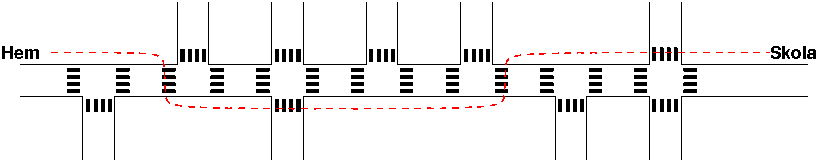
\includegraphics[width=0.8\textwidth]{skolvag.png}
\end{center}
\caption{The dotted line shows Cissi's optimal path in the first example.}
\end{figure}

\noindent
Cissi is walking from her home to school, following a long street going from the west to the east.
On her way, she passes a number of street crossings where the crossing street either goes north (\texttt{N}), south (\texttt{S}) or both (\texttt{B}).
At every street crossing, there are crosswalks on both the crossing streets and the main street (see the figure above), and she can only cross the street on the crosswalks.

Her home is to the north of the main street, furthermost to the west.
The school is to the north of the main street, furthermost to the east.
Write a program that helps Cissi compute the smallest number of streets that she must cross on her path to school.

\section*{Input}
The input contains a single line with at most $1\,000$ letters, each of which is {\tt N}, {\tt S} or {\tt B}.
The letters describe the crossing streets exactly in the order Cissi will pass them on her way to school.

\section*{Output}
A single line with an integer, the smallest number of streets Cissi needs to cross.

\section*{Scoring}
Your solution will be tested on a set of test case groups.
To get the points for a group, you need to pass all the test cases in the group.

\noindent
\begin{tabular}{| l | l | p{10cm} |}
\hline
Group & Points & Constraints \\ \hline
  $1$    & $40$        & There are at most $20$ crossing streets \\ \hline 
  $2$    & $60$        & No further constraints. \\ \hline 
\end{tabular}

